\chapter{Using Experts for Design}

\label{ch:contracat}

Genuinely varied, realistic data is necessary to create models that are robust to minor variations. 
%
However, equally robust evaluation methodologies are important in ascertaining the quality of the data. 
%
Current methods focus on quantitative assessments that may inadvertently assess the \textit{annotation}, but not the \textit{generation}, quality of a dataset.  
%
Since most datasets are evaluated on the same types of data---\squad{} test data is comparable to the training data---the linguistic variation of a dataset is not readily captured by standard quantitative metrics like accuracy or \fone{}.
%
Furthermore, a model that has memorized several key answers upon which it is then tested is not necessarily \textit{learning}.
%
A raw analysis of data overlap appears this is at least partially a problem~\citep{lewis2020question}.    
%
Datasets meant to effectively and robustly evaluate trained datasets can determine how much of a problem this poses \textit{ex-post-facto}.  

As one solution to this limitation, Checklist~\citep{ribeiro2020beyond} created a task-agnostic methodology for testing NLP models.
%
We extend this work to a specific task: testing coreference~\citep{soon2001machine} in machine translation. %in Section~\ref{sec:propeval}.  
%
The dataset we create is \textit{designed} by experts: specifically native German and native English speakers, even if the methodology is \textit{automated}.
%
While a similar dataset of the same size could be created without knowledge of either language, the templates used as test data would prove be nonsensical or unnatural.  

\section{Meaningful Model Evaluation in Machine Translation}
\label{sec:propeval}

%Due to the intrinsic evaluation of many datasets, higher standards of evaluation would better understand the strength of machine learning models, and indirectly the data used to train them.
%

%


Machine translation is a classic \nlp{} task with immediate real-world application.
%
Its a complex task that requires diverse linguistic knowledge and data in multiple languages.
%
Classic datasets were often gathered through extensive collaboration with experts.
%
However, recent ones are often created through crowd-sourcing or automatic methods. 
%
Therefore, this is an area well-suited to our evaluation techniques.  

We focus on German-English coreference resolution as a representative task.  
%
The seemingly straightforward translation of the English pronoun \textit{it} into German requires knowledge at the syntactic, discourse and world knowledge levels for proper pronoun coreference resolution (\coref{}).
%
A German pronoun can have three genders, determined by its antecedent: masculine (\emph{er}), feminine (\emph{sie}) and neuter (\emph{es}).
%
The nuance of this work requires native knowledge of both English and German.  

Accuracy in machine translation is at an all-time high with the rise of neural architectures~\citep{wu2016googles}; but does accuracy alone suffice?  
%
Previous work~\citep{hardmeier2010modelling,miculicich-werlen-popescu-belis-2017-validation,mueller2018} proposed evaluation methods for specifically pronoun translation. 
%
This has been of special interest in context-aware neural machine translation (\nmt{}) models that are capable of using discourse-level information.
%
Despite promising results, the question remains: 
Are transformers \citep{vaswani2017attention} truly \textit{learning} this task, or are they exploiting simple heuristics to make a coreference prediction?
% 
To empirically answer this question, we propose extending ContraPro~\citep{mueller2018}---a contrastive challenge set for automatic English$\rightarrow$German pronoun translation evaluation\footnote{ContraPro is described in detail in Section~\ref{sec:contrapro}}---by making small adversarial changes in the contextual sentences.\footnote{Equal effort between Denis Peskov, Benno Krojer, Dario Stojanovski, and supervised by Alex Fraser. 2020. In International Conference on Computational Linguistics \\ Peskov is responsible for part of template design, selecting concrete nouns for the templates, paper writing, and the video.}

Our adversarial attacks on ContraPro show context-aware Transformer \nmt{} models can easily be misled by simple and unimportant changes to the input.
%
However, interpreting the results obtained from adversarial attacks can be difficult. 
%
In our case, trivial changes in language cause incorrect predictions, but both the changes and the prediction would not be noticed by somebody without a mastery of German.  
%
Positive results will show that \nmt{} uses brittle heuristics to solve \coref{}, since trivial changes in pronouns and nouns should not fool a coreference corpus like ContraPro.
%
However, modifying ContraPro alone will not test specific phenomena and will only demonstrate a broad dependence on heuristics.  

For this reason, we propose a new dataset, created from templates (Section~\ref{sec:template}), to systematically evaluate which heuristics are being used in coreferential pronoun translation.  
%
Inspired by previous work on \coref{}~\citep{raghunathan2010multi,lee2011stanford}, we will create templates tailored to evaluating the specific steps of an idealized \coref{} pipeline. 
%
We will call this collection \contracat{}, \textbf{C}ontrastive \textbf{C}oreference \textbf{A}nalytical \textbf{T}emplates. 
%
The construction of templates is controlled, enabling us to easily create large number of coherent test examples and provide unambiguous conclusions about the \coref{} capabilities of \nmt{}. 
%
While this methodology depends on automation, a technique called into question in Chapter \ref{ch:unspecialized}, the templates are written in collaborations between a native German speaker and native English speakers. 
%
Since automation is subject to quality control issues, this level of expertise is necessary if the adversarial dataset is to be reflective of actual language used by English and German speakers.
%
The procedure used in creating these templates can be adapted to many language pairs with little effort.
%
We also propose a simple data augmentation approach using fine-tuning. 
%
This methodology should not change the way \coref{} is being handled by \nmt{} and support the hypothesis that automated data techniques have limited applicability.  
%
We will publicly release a new dataset, ContraCAT, and the adversarial modifications to ContraPro.

ContraCAT applies only to coreference, but the investigation of heuristics is an important research direction in \nlp{}, that can quantify the issues noted with automatic and crowd-sourced datasets (Chapter~\ref{ch:unspecialized}), even if experts are unavailable ()Chapter~\ref{ch:hybrid}).
%
Heuristics perform well if there are underlying data limitations; this implies that the training data and the evaluation data resemble one another in superficial ones.
%
Therefore, exposing the brittleness in current datasets motivates the need for higher-quality evaluation data---to observe this limitation---and varied training data---to overcome it.  

We introduce coreference resolution as a task in Section~\ref{sec:mtbg}, the idealized coreference pipeline in Section~\ref{sec:mtbg}, and the transformer model in Section~\ref{sec:contracatmodel}.  
We discuss ContraPro in Section~\ref{sec:contrapro}, and explain our proposed templates in Section~\ref{sec:templates}.


\section{Why is Coreference Resolution Relevant?}
\label{sec:mtbg}


Evaluating discourse phenomena is an important first step in evaluating \abr{mt}.  
%
Apart from document-level coherence and cohesion, anaphoric pronoun translation has proven to be  an important testing ground for the ability of context-aware \nmt{} to model discourse. 
%
Anaphoric pronoun translation is the focus of several works in context-aware \nmt{}~\citep{bawden-etal-2018-evaluating,voita2018anaphora,stojanovski-fraser-2018-coreference,miculicich2018documentnmt,voita2019good,maruf2019selective}. 



\begin{table}[t]
	\centering
	\begin{tabular}{p{4cm} p{8cm}}
		\tikzmark{a} Start:  \newline Original sentence & The cat and the actor were hungry.  
		\newline
		It (?) was hungrier. \\
		\hline
		\tikzmark{b} Step 1: \newline  \stepone{} & The \textbf{cat} and the \textbf{actor} were hungry.  
		\newline
		It (?) was hungrier. \\
		\hline
		\tikzmark{c} Step 2: \newline  \steptwo{} & The cat and the actor were hungry. 
		\newline
		\textbf{It} was hungrier. \\
		\hline
		\tikzmark{d} Step 3: \newline \stepthree{} & Der Schauspieler und die Katze waren hungrig.
		\newline
		Er / \textbf{Sie} / Es   war hungriger.  \\
	\end{tabular}
	\begin{tikzpicture}[overlay, remember picture, yshift=.25\baselineskip, shorten >=2pt, shorten <=2pt, very thick]
	\draw [orange, ->] ({pic cs:a}) [bend right] to ({pic cs:b});
	\draw [orange, ->] ({pic cs:b}) [bend right] to ({pic cs:c});
	\draw [orange, ->] ({pic cs:c}) [bend right] to ({pic cs:d});
	
	\end{tikzpicture}
	
	\caption{A hypothetical \textsc{cr} pipeline that sequentially resolves and translates a pronoun.}
	\label{tab:corefpipeline}
\end{table}


The choice of an evaluation metric for \textsc{cr} is nontrivial. 
%
\textsc{bleu}-based evaluation is insufficient for measuring improvement in \textsc{cr}~\citep{hardmeier2012discourse} 
% and has led to custom variation
without carefully selecting or modifying test sentences for pronoun translation~\citep{voita2018anaphora,stojanovski-fraser-2018-coreference}.
%
Alternatives to \textsc{bleu} include $F_1$, partial credit, and oracle-guided approaches~\citep{hardmeier2010modelling,guillou-hardmeier-2016-protest,miculicich-werlen-popescu-belis-2017-validation}. 
%
However, \citet{guillou-hardmeier-2018-automatic} show that these metrics can miss important cases and propose semi-automatic evaluation. 
%
In contrast, our evaluation will be \textit{completely} automatic.  
%
We focus on scoring-based evaluation~\citep{sennrich-2017-grammatical}, which works by creating contrasting pairs and comparing model scores. 
%
Accuracy is calculated as how often the model chooses the correct translation from a pool of alternative incorrect translations.
%
This is an evaluation metric applicable for multiple forms of \textit{generated} \nlp{} data.

Our work is related to adversarial datasets for testing robustness used in  Natural Language Processing tasks such as  studying gender bias~\citep{zhao2018gender,rudinger2018gender,stanovsky-etal-2019-evaluating}, natural language inference \citep{glockner-etal-2018-breaking} and classification \citep{wang2019natural}.
% wang2019 mentions works about synonym replacement 


\section{Do Androids Dream of Coreference Translation Pipelines?}
\label{sec:corefpipeline}

Imagine a hypothetical coreference pipeline that generates a pronoun in a target language, as illustrated in  Table~\ref{tab:corefpipeline}.
%
\textbf{First}, markables (entities that can be referred to by pronouns) are tagged in the source sentence (we restrict ourselves to concrete entities as concepts are incompatible with many verbs). 
%
Then, the subset of animate entities are detected, and human entities are separated from other animate ones (since \textit{it} cannot refer to a human entity).
%
\textbf{Second}, coreferences are resolved in the source language. 
%
This entails addressing phenomena such as world knowledge, pleonastic \textit{it}, and event references.  
%
\textbf{Third}, the pronoun is translated into the target language. This requires selecting the correct gender given the referent (if there is one), and selecting the correct grammatical case for the target context (e.g., accusative, if the pronoun is the grammatical object in the target language sentence).

%Thus, the
This idealized
pipeline would produce the correct pronoun in the target language. 
%
The coreference steps resemble the rule-based approach implemented in Stanford Core\textsc{nlp}'s CorefAnnotator~\citep{raghunathan2010multi,lee2011stanford}. 
%
However, \nmt{} models are unable to decouple
the individual steps
of this pipeline. 
%
We propose to isolate each of these 
steps through targeted examples.


\section{Model}
\label{sec:contracatmodel}

% \afcomment{TODO: fix ContraPRO to be ContraPro everywhere}
% \dscomment{Fixed, but keeping it as a reminder.}

We use a transformer model (Background Section~\ref{sec:seq2seq}) for all experiments and train a sentence-level model as a baseline.
%
The context-aware model in our experimental setup is 
a concatenation model~\citep{tiedemann2017neural} (\textsc{concat}) which is trained on a concatenation of consecutive sentences.
%
\textsc{concat} is a standard transformer model and it differs from the sentence-level model only in the way that the training data is supplied to it.\footnote{The training examples for this model are modified by prepending the previous source and target sentence to the main source and target sentence. 
	%
	The previous sentence is separated from the main sentence with a special token $<$SEP$>$, on both the source and target side. 
	%
	This also applies to how we prepare the ContraPro and \contracat{} data. 
	%
	We train the concatenation model on OpenSubtitles2018 data prepared in this way. 
	%
	We remove documents overlapping with ContraPro.}
% We incorporate contextual information into the model by concatenating consecutive sentences~\cite{tiedemann2017neural}.   
%




\section{Adversarial Attacks}
ContraPro, a contrastive challenge set, has limitations and our methodology for creating our own dataset addresses them.

\subsection{About ContraPro}
\label{sec:contrapro}

ContraPro is a contrastive challenge set  for English$\rightarrow$German pronoun translation evaluation. 
%
This dataset uses an  \textit{automated} approach, discussed in Chapter~\ref{ch:unspecialized}.
%
The automatic nature makes it subject to manipulation and prevents it from fully elucidating the limitations of neural coreference resolution. 
%
The set consists of English sentences containing an anaphoric pronoun ``it'' and the corresponding German translations (e.g., ``Give me your hand, ah, it's soft and hot, and it feels pleasant''$\overrightarrow{}$``Gib deine Hand, ah, sie ist weich und warm, und wohlig fühlt sie sich an.'').
%
It contains three contrastive translations, 
differing based on the gender of the translation of \textit{it}: \textit{er}, \textit{sie}, or \textit{es}.
%
The challenge set artificially balances the  amount of sentences where \textit{it} is translated to each of these three German pronouns.
%
The appropriate antecedent may be in the main sentence or in a previous sentence. 
%
For evaluation, a model needs to produce scores for all three possible translations, 
which are compared against ContraPro's gold labels.


We create automatic adversarial attacks on ContraPro that modify theoretically inconsequential parts of the context sentence before the occurrence of \emph{it}. 
%
Contrary to the expectation that a transformer model would be able to handle inconsequential priming, coreference accuracy degrades in all adversarial attacks.


\subsection{Adversarial Attack Generation}
\label{sec:templates}

Our three modifications are:

\begin{enumerate}[noitemsep]
	\item \textbf{Phrase Addition}: Appending and prepending phrases containing implausible antecedents:
	\vspace{.1cm}
	The Church is merciful \emph{\underline{but that's not the point}}. It always welcomes the misguided lamb.
	\vspace{.2cm}
	
	\item \textbf{Possessive Extension}: Extending original antecedent with possessive noun phrase:
	\vspace{.1cm}
	I hear \sout{her} \emph{\underline{the doctor's}} voice! It resounds to me from heights and chasms a thousand times!
	
	\vspace{.2cm}
	\item \textbf{Synonym Replacement}: Replacing original German antecedent with synonym of different gender (note: \emph{der Vorhang} (masc.) and \emph{die Gardine} (fem.) are synonyms meaning \emph{curtain}):
	
	The curtain rises. It rises. $\rightarrow$ \sout{Der Vorhang} \emph{\underline{Die Gardine}} geht hoch. \sout{Er} \emph{\underline{Sie}} geht hoch.
\end{enumerate}


Phrase Addition can be applied to all 12,000 ContraPro examples. 
%
The second and third attack can only be applied to 3,838 and 1,531 examples, due to the required sentence contingencies.  

\subsubsection{Phrase Addition}
%As shown in the example in Table~\ref{tab:attacks} 
This attack modifies the previous sentence
by appending phrases such as ``\dots{}\textit{but he wasn't sure}'' and also prepending phrases such as ``\emph{it is true}:\dots{}''.
%
A range of other simple phrases can be used, which we leave out for simplicity.  All phrases we tried provided lower scores.
%
These attacks either introduce a human entity or an event reference \textit{it} (e.g.,  \textit{``it is true''}) which are both not plausible antecedents for the anaphoric \textit{it}.
% In the case of  ``it is true:..." we also created attacks with  ``that is true" and attacks that append "...and it is true.". This measures the difference between ``it'' and ``that'' and the role of distances in anaphoric pronoun translation.  
% are these details important?

\subsubsection{Possessive Extension}
This attack introduces a new human entity by extending the original antecedent \emph{A} with a possessive noun phrase e.g., ``\textit{the woman's A}''. 
%
Only two-thirds of the 12,000 ContraPro sentences are linked to an antecedent phrase. Grammar and misannotated antecedents exclude half of the remaining phrases.
% For example regarding grammar, an antecedent in ContraPro such as \textit{this one/der hier}, cannot be extended with"\textit{the woman's\dots}".
% \dscomment{Is this necessary?}
We put \textsc{pos}-tag constraints on the antecedent phrases before extending them. 
% with possessive Noun Phrases. 
%
This filters our subset to 3,838 modified examples. 
%
Our possessive extensions can be humans (\textit{the woman's}), organisations (\textit{the company's}) and names (\textit{Maria's}).

\subsubsection{Synonym Replacement}
This attack modifies the original German antecedent by replacing it with a German synonym of a different gender. 
%
For this we first identify the English antecedent and its most frequent synset in WordNet \citep{miller1995wordnet}.
% , as a word sense disambiguation baseline. 
% no further reference about this
%
We obtain a German synonym by mapping this WordNet synsets to GermaNet \citep{hamp-feldweg-1997-germanet} synsets.
%
Finally, we modify the correct German pronoun translation to correspond to the gender of the antecedent synonym.

Approximately one quarter of the nouns in our ContraPro examples are found in GermaNet.  
In 1,531 cases, a synonym of different gender could be identified. 

Understanding the pronoun/noun relationship is needed to score well on the Synonym Replacement attack. This attack gets to the core of whether \nmt{} uses \coref{} heuristics instead.

We evaluate a random sample of 100 auto-modified examples as a quality control metric.  
%
There are 11 issues with semantically-inappropriate synonyms. 
%
Overall, in 14 out of 100 cases, the model switches from correct to incorrect predictions because of synonym-replacement.
%
Only 4 out of these 14 cases come from the questionable synonyms, showing that the drop in ContraPro scores is meaningful.

\begin{figure}[t!]
	\centering
	\includegraphics[width = \linewidth]{\figfile{F1.pdf}}
	\caption{Results with the sentence-level Baseline and \textsc{concat} on ContraPro and three adversarial attacks. 	
		The adversarial attacks modify the context, therefore the Baseline model's results on the attacks are unchanged and we omit them.  \textbf{Phrase}: prepending ``it is true: \dots''. \textbf{Possessive}:  replacing original antecedent \emph{A}  with ``Maria's \emph{A}''. \textbf{Synonym}: 
		replacing the original antecedent with different-gender synonyms.  Results for Phrase Addition are computed based on all 12,000 ContraPro examples, while for Possessive Extension and Synonym Replacement we only use the suitable subsets of 3,838 and 1,531 ContraPro examples. 
	}
	\label{fig:contrapro}
\end{figure}



\subsubsection{Evaluating Adversarial Attacks }


Intuitively, the adversarial attacks should not contribute to large drops in scores, since  no meaningful changes are being made.
%
If the model accuracy drops some, but not all the way to the original sentence-level baseline (Section~\ref{sec:contracatmodel}),  we can conclude that the concatenation model handles \coref{}, but likely with brittle heuristics.
%
If the model accuracy drops all the way to the baseline, then the model is memorizing the inputs.
%
These results can expose potential issues with the model, but it will still be difficult to pinpoint the specific problems. 
%
This reveals a larger issue with pronoun translation evaluation that cannot be addressed with simple adversarial attacks on existing general-purpose challenge sets. 
%
We propose \contracat{}, a more systematic approach that targets each of the previously outlined \coref{} pipeline steps with data synthetically generated from corresponding templates.

Automatic adversarial attacks offer less freedom than templates as many systematic modifications cannot be applied to the average sentence.
%
Thus, our \contracat{} templates will be built on the hypothetical coreference pipeline in Section~\ref{sec:corefpipeline} that target each of the three steps:
%
i) \stepone{}, ii) \steptwo{} and iii) \stepthree{}. 
%Step ii) (Coreference resolution) is targeted in more detail with additional sub-steps.
%
Our minimalistic templates draw entities from sets of animals, human professions~\citep{mccoy2019right},
foods, and drinks, along with associated verbs and attributes. 
%
We use these sets to fill slots in our templates. 
%
Animals and foods are natural choices for subject and object slots referenced by \emph{it}.
%
Restricting our sets to interrelated concepts with generically applicable verbs---all animals eat and drink---ensures semantic plausibility.
%
Other object sets, such as buildings, would cause semantic implausibility with certain verbs.  

\subsubsection{Template Generation}
\label{sec:template}

\begin{table}[t]
	\small
	\centering
	\begin{tabular}{p{4.5cm} p{9cm} }
		\textbf{Template Target} & \textbf{Example} \\
		\hline
		
		\noalign{\vskip 2mm} 
		\textbf{Priors} & \\
		Grammatical Role & The \emph{\textbf{cat}} ate the \emph{\textbf{egg}}. It (\cat{}/{\textit{egg}}) was big. \\
		Order & I stood in front of the \emph{\textbf{cat}} and the \emph{\textbf{dog}}. It (\cat{}/\textit{dog}) was big. \\
		Verb & Wow! She unlocked it. \\
		
		
		\noalign{\vskip 2mm} 
		\rowcolor{gray!25}
		\textbf{\stepone{}} & \\
		\rowcolor{gray!25}
		Filter Humans & The \textit{\textbf{cat}}  and the \textit{actress} were happy. However it (\cat{}) was happier.  \\
		
		\noalign{\vskip 2mm} 
		\textbf{\steptwo{}} & \\
		Lexical Overlap & The \textit{\textbf{cat}} ate the apple and the \textit{owl} drank the water. It (\cat{}/ \textit{dogFir}) ate the apple quickly. \\
		World Knowledge & The \textit{\textbf{cat}} ate the \textit{cookie}. It (\cat{}) was hungry. \\
		% \dscomment{Changed is hungry to was hungry for past tense consistency.}
		Pleonastic it & The \emph{cat} ate the \emph{sausage}. It was raining. \\
		Event Reference  & The \emph{cat} ate the \emph{carrot}. It came as a surprise. \\
		
		\rowcolor{gray!25}
		\noalign{\vskip 2mm} 
		\textbf{\stepthree{}} & \\
		\rowcolor{gray!25}
		Antecedent Gender &
		I saw a \textit{\textbf{cat}}. It(\cat{}) was big. 
		$\rightarrow$
		\newline
		Ich habe eine Katze gesehen. Sie (\cat{}) war gro{\ss}.
	\end{tabular}
	\caption{Template examples targeting different \coref{} steps and substeps. 
		% We used sets of associated nouns, i.e.,, \{dog, cat, pig, 
		%\} for Animals.
		% is this important here? In any case, it is not clear 
		For German, we create three versions with \emph{er}, \emph{sie}, or \emph{es} as different translations of \emph{it}.
		% For the German translation we created three versions of the template with \emph{er}, \emph{sie}, or \emph{es} as different translations of \emph{it}. 
		% For consistency with how our model is trained, sentences are separated by $<$SEP$>$.
		% moved this to Model
	}
	\label{tab:templates}
\end{table}

Our templates consist of a \emph{previous sentence} that introduces at least one entity and a \emph{main sentence} containing the pronoun \emph{it}.
%
We use contrastive evaluation to judge anaphoric pronoun translation accuracy for each template; we create three translated versions for each German gender corresponding to an English sentence, e.g., \textit{``The cat ate the egg. It rained.''} and the corresponding \textit{``Die Katze hat das Ei gegessen. \emph{Er/Sie/Es} regnete''}.
%
To fill a template, we only draw pairs of entities with two different genders, i.e., for animal $a$ and food $f$: gender($a$) $\neq$ gender($f$). 
%
This way we can determine whether the model has picked the right antecedent.

First, we will create templates that analyze priors of
the model for choosing a pronoun when no correct translation is obvious. 
%
Then, we will create templates with correct translations, guided by the three broad coreference steps.
% \dscomment{This paragraph may not be necessary. We can mention it in Priors.}
Table~\ref{tab:templates} provides examples for our templates.


% \subsubsection{Biases}
\subsubsection{Priors}

% \afcomment{I added the next sentence, I am bit concerned that people might get confused between the priors and the other templates, which are really different. In fact, even after adding this sentence I am still concerned about this.}

Our templates that test prior biases do not have a correct answer, but help to understand the model's biases.
%
We will expose three priors with our templates: i) grammatical roles prior (e.g., subject)
ii) position prior  (e.g., first antecedent) and iii) a general prior if no antecedent and only a verb is present.

For i), we will create a Grammatical Role template where both subject and object are valid antecedents. 
%

For ii), we will create a Position template where two objects are enumerated as shown in Table~\ref{tab:templates}. 
%
We will create an additional example where the entities order is reversed and test if there are priors for specific nouns or alternatively positions in the sentence.  

For iii), we will create a Verb template, expecting that certain transitive verbs trigger certain object gender choice. 
%
We will use 100 frequent transitive verbs and create sentences such as the example in Table~\ref{tab:templates}.


\subsubsection{Markable Detection with a Humanness Filter}
Before doing the actual \coref{}, the model will need to identify all possible entities that \textit{it} can refer to. 
%
We will construct a template that contains a human and animal which are in principle plausible antecedents, if not for the condition that \emph{it} does not refer to people. 
%
For instance, the model should always choose \emph{cat} in \textit{`` The \emph{actress} and the \emph{cat} are hungry. However \emph{it} is hungrier.''}. 

\subsubsection{Coreference Resolution}
Having determined all possible antecedents, the model will have to choose the correct one, relying on semantics, syntax, and discourse.
%
The pronoun \textit{it} can in principle be used as an \emph{anaphoric} (referring to entities), \emph{event reference} or \emph{pleonastic} pronoun \citep{loaiciga-etal-2017-disambiguating}.
%
For the anaphoric \textit{it}, we identify two major ways of identifying the antecedent: lexical overlap and world knowledge.  
%
Our templates for these categories are meant to be simple and solvable.  

\textbf{Overlap}: Broadly speaking the subject, verb, or object can overlap from the previous sentence to the main sentence, as well as combinations of them. 
%
This gives us five templates: i) subject-overlap ii) verb-overlap iii) object-overlap iv) subject-verb-overlap and v) object-verb-overlap.

%
We always use the same template for the context sentence, e.g., \textit{``The \textbf{cat} ate the apple and the \textbf{owl} drank the water.''}. 
%
For the object-verb-overlap we would then create the main sentence \textit{``It ate the apple quickly.''} and expect the model to choose \emph{cat} as antecedent.
%
To keep our overlap templates order-agnostic, we vary the order in the previous sentence by also creating \textit{``The \textbf{owl} drank the water and the \textbf{cat} ate the apple.''}

\textbf{World Knowledge}: \coref{} has been traditionally seen as challenging as it requires  world knowledge.
%
Our templates will test simple forms of world knowledge by using attributes that either apply to animal or food entities, such as \textit{cooked} for food or \textit{hungry} for animals.
%
We then evaluate whether the model chooses e.g., \emph{cat} in \textit{``The \textbf{cat} ate the cookie. It was hungry.''}
%
The model occasionally predicts answers that require world knowledge, but most predictions are guided by a prior for choosing the neuter \emph{es} or a prior for the subject.

% \bkcomment{should i do this?:}
% To see if the model exhibits world knowledge when the bias is not triggered as much, we construct a less natural but still plausible template: ``I looked at the \emph{cat} and the \emph{ice cream}. It had a sweet taste''. This leads to XXX.
% \dscomment{Commenting this for now.}

\textbf{Pleonastic and Event Templates}: For the other two ways of using \emph{it}, event reference and pleonastic-it, we again create a default previous sentence (\textit{``The \textbf{cat} ate the \emph{apple}.'')}. 
%
For the main sentence, we used four typical pleonastic and event reference phrases such as \textit{``It is a shame''} and \textit{``It came as a surprise''}.  
%
We expect the model to correctly choose the neuter \emph{es} as a translation every time.  

\subsubsection{Translation to German}
\label{gender_template}

After \coref{}, the decoder has to translate from English to German.
%
In  our contrastive scoring approach the translation of the English antecedent to German is already given.
%
However the decoder is still required to know the gender of the German noun to select between \emph{er}, \emph{sie} or, \emph{es}. 
%
We will test this with a list of concrete nouns selected from \citet{Brysbaert2014ConcretenessRF}, which we filter for nouns that occur more than $30$ times in the training data. 
%
This selects $2051$ nouns that are substituted for $N$ in: \textit{``I saw a $N$. It was \{big, small\}.''.}

\subsection{Results} \label{template_results}

The \textsc{concat} model becomes less accurate when actual \coref{} is required. 
%
It frequently falls back to choosing the neuter \emph{es} or preferring a position (e.g., first of two entities) for determining the gender.
%
For \emph{Markable Detection} the model always predicts the neuter \emph{es} regardless of the actual genders of the entities.

% When the model was tested to do \coref{} by looking at different types of overlaps, it failed to recognize the overlap and had instead a general preference for one of the two clauses. 
In the Overlap template, the model fails to recognize the overlap and has a general preference for one of the two clauses.
%
For instance in the case of verb-overlap, the model had a solid accuracy of $64.1\%$ if the verb overlapped from the first clause (\textit{``The cat ate and the dog drank. It ate a lot.''}) but a weak accuracy of $39.0\%$ when the verb overlapped from the second clause (\textit{``The cat ate and the dog drank. It drank a lot.''.}) 
%
The overall accuracy for the overlap templates is $47.2\%$, with little variation across the types of overlap. 
% \bkcomment{should i report overall score here or score for all 5 overlaps?}
% Surprisingly 
Adding more overlap, e.g., by overlapping both the verb and object (\textit{``It ate the apple happily''}), yields no improvement. 
%
Overall, the model pays very little attention to overlaps when resolving pronouns.
% \dscomment{not sure if this is good or not}

\begin{figure}[t!]
	\centering
	\includegraphics[width = \linewidth]{\figfile{F2.pdf}}
	\caption{Results comparing the sentence-level baseline to \textsc{concat} on Contra\abr{cat}.  Pronoun translation pertaining to World Knowledge and language-specific Gender Knowledge benefits the most from additional context.}
	\label{fig:templates}
\end{figure}


We also see weak performance for world knowledge. An accuracy of $55.7\%$ is slightly above the heuristic of randomly choosing an entity ($=50.0\%$).
% \dscomment{Check}
% This means there is some small world knowledge in the model, however not enough to solve the task.
With a strong bias for the neuter \emph{es}, the model has a high accuracy of $96.2\%$ for event reference and pleonastic templates, where \emph{es} is always the correct answer.
%
Based on the strong performance on the Gender template in Section~\ref{gender_template}, we conclude the model consistently memorized the gender of concrete nouns.
%
Hence, \coref{} mistakes stem from Step 1 or Step 2, suggesting that the model failed to learn proper \coref{}.



\begin{table}[ht]
	\small
	\centering	
	\begin{tabular}{l l}
		
		\multicolumn{2}{l}{\textbf{Antecedent-free augmentation}} \\
		\textit{Source} &
		You let me worry about that. $<$SEP$>$ How much you take for \underline{it}? \\
		\textit{Reference} &
		Lassen Sie das meine Sorge sein. $<$SEP$>$ Wie viel kostet \underline{er}? \\
		\textit{Augmentation 1} &
		Lassen Sie das meine Sorge sein. $<$SEP$>$ Wie viel kostet \underline{sie}? \\
		\textit{Augmentation 2} &
		Lassen Sie das meine Sorge sein. $<$SEP$>$ Wie viel kostet \underline{es}? \\
	\end{tabular}
	\caption{Examples of training data augmentations. The source side of the augmented examples remains the same.}
	\label{table:manual-examples-augmentations-main}
\end{table}

\section{Augmentation}
\label{sec:augment}

We present an approach for augmenting ContraPro to improve \textsc{cr}.    
%
Augmentation systematically expands the data to improve a model's robustness~\citep{kafle2017data}.
%
While challenging for \textsc{nlp},  we focus on a narrow problem which lends itself to easier data manipulation. 
%
Figure~\ref{fig:templates} shows that our model is capable of modeling the gender of nouns.
%
However, they also show a strong  prior for translating \textit{it} to \textit{es} and very little \coref{} capability.
%
Our goal with the augmentation is to alter the prior and test if this can improve \coref{} in the model.


We augment our training data 
and call it Antecedent-free augmentation (\textsc{afa}).
%
We identify candidates for augmentation as sentences where a coreferential \textit{it} refers to an antecedent not present in the current or previous sentence  (e.g., \textit{I told you before. $<$SEP$>$ \underline{It} is red.} $\rightarrow$ \textit{Ich habe dir schonmal gesagt. $<$SEP$>$ \underline{Es} ist rot.}).
%
We create augmentations by adding two new training examples where the gender of the German translation of ``it'' is modified 
(e.g., the two new targets are ``\textit{Ich habe dir schonmal gesagt. $<$SEP$>$ \underline{Er} ist rot.}'' and ``\textit{Ich habe dir schonmal gesagt. $<$SEP$>$ \underline{Sie} ist rot.}'').
The source side remains the same.
%
Table~\ref{table:manual-examples-augmentations-main} provides an additional example.
%
Antecedents and coreferential pronouns are identified using a \coref{} tool \citep{clark2016deep,clark-manning-2016-improving}.
%
We fine-tune our  already trained concatenation
model on a dataset consisting of the candidates and the augmented samples. 
%
As a baseline, we fine-tune on the candidates to confidently say that any potential improvements come from the augmentations. 


\subsection{Results}
Results for adversarial attacks on ContraPro and on our templates are independent and are discussed separately.  

\begin{figure}[ht!]
	\centering
	\includegraphics[width = \linewidth]{\figfile{F3.pdf}}
	\caption{Results comparing unaugmented and augmented \textsc{concat} on ContraPro and same 3 attacks as in Figure~\ref{fig:contrapro}. Results with non-augmented \textsc{concat} are the same as Figure \ref{fig:contrapro}.}
	\label{fig:augmentation-contrapro}
\end{figure}

\subsubsection{Adversarial Attacks}

\textsc{afa} provides large improvements, scoring 85.3\% on ContraPro (Figure~\ref{fig:augmentation-contrapro}).
%
The \textsc{afa} baseline  (fine-tuning on the augmentation candidates only) improves by 1.94\%, presumably because many candidates consist of coreference chains of ``it'' and the model learns they are important for coreferential pronouns. However, the improvement is small compared to \textsc{afa}. 
% translation. 



Prediction accuracy on \textit{er} and \textit{sie} is substantially increased, suggesting that the augmentation removes the strong bias towards \textit{es}. %Templates provide further evidence about this. 
%
Although, the adversarial attacks lower \textsc{afa} scores, 
in contrast to \textsc{concat}, the model is more robust and the accuracy degradation is substantially lower (except on the synonym attack).
% 
We experiment with different learning rates during fine-tuning and 
present results with the \textsc{lr} that obtain 
the  best  baseline ContraPro score.
%
Furthermore, \textsc{concat}  and \textsc{afa} obtain $31.5$  and $32.2$ \textsc{BLEU} on ContraPro, showing that this fine-tuning procedure, which is tailored to pronoun translation, does not lead to any degradation in overall translation quality.

\subsubsection{Templates}



The prior over gender pronouns is more evenly spread and not concentrated on \textit{es}.
%
This provides for a more even distribution on the Position and Role Prior template.

The augmented model has higher accuracy on markable detection, improving by $27.6\%$. 
%
Results for  the templates are in Figure~\ref{fig:augmentation-templates}.




\begin{figure}[!h]
	\centering
	\includegraphics[width = \linewidth]{\figfile{F4.pdf}}
	
	\begin{comment}
	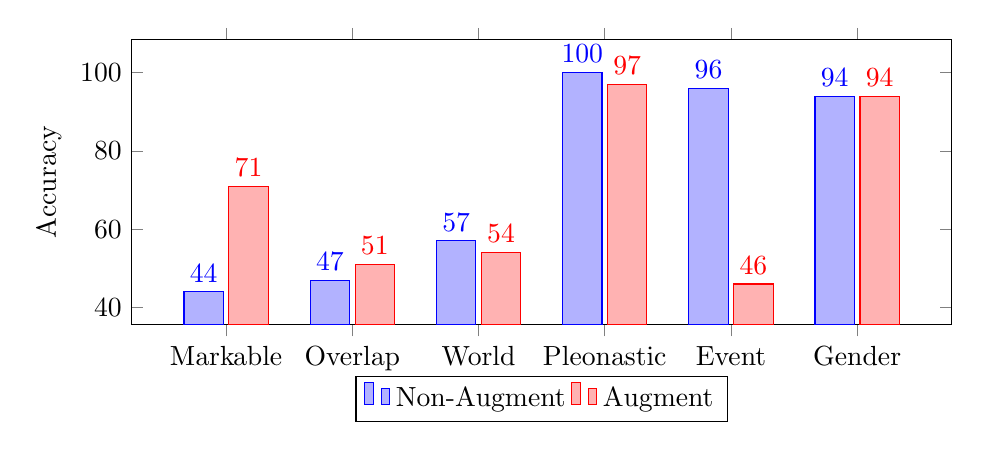
\begin{tikzpicture}
	\begin{axis}[
	ybar,
	enlargelimits=0.15,
	legend style={at={(0.5,-0.18)},
	anchor=north,legend columns=-1},
	ylabel={Accuracy},
	symbolic x coords={Markable,Overlap,World,Pleonastic,Event,Gender},
	xtick=data,
	nodes near coords,
	nodes near coords align={vertical},
	height=5.2cm,
	width=12cm,
	bar width=0.5cm,
	]
	\addplot coordinates {(Markable,44) (Overlap,47) (World,57) (Pleonastic,100) (Event,96) (Gender,94)};
	\addplot coordinates {(Markable,71) (Overlap,51) (World,54) (Pleonastic,97) (Event,46) (Gender,94)};
	\legend{Non-Augment,Augment}
	\end{axis}
	\end{tikzpicture}
	\end{comment}
	% \caption{Augmentation improves \textsc{Concat}'s pronoun translations on ContraCAT.  We speculate that this is explained by a readjusting of the prior. }
	\caption{ContraCAT results with unaugmented and augmented \textsc{concat}. We speculate that readjusting the prior over genders in augmented \textsc{concat} explains the improvements on Markable and Overlap.}
	\label{fig:augmentation-templates}
\end{figure}

% Considering our augmentation approach, 
No improvements are observed on the World Knowledge template.
Pleonastic cases are still accurate, although not perfect as with \textsc{concat}. 
% The shift in prior distribution over pronouns causes a small number of mistakes. 
The Event template identifies a systematic issue with our augmentation. We presume this is due to the \coref{} tool marking cases where \textit{it} refers to events. 
%
We do not  apply any filtering and augment these cases as well,
thus creating wrong examples (an event reference \textit{it} cannot be translated to \textit{er} or \textit{sie}). 
%
As a result, the scores are significantly lower compared to \textsc{concat}. 
%
This issue with our model is not visible on ContraPro and the adversarial attacks results. In contrast, the Event template easily identifies this problem.

\textsc{afa} has a similar accuracy to the unaugmented baseline on the Gender template. 
%
However,
despite increasing by 3.8\%, results on Overlap are still underwhelming. 
%
Our analysis shows that augmentation helps in changing the prior. 
%
We believe this provides for improved \coref{} heuristics which in turn provide for an improvement in coreferential pronoun translation. 
%
Nevertheless, the Overlap template shows that augmented models still do not solve \coref{} in a fundamental way.


\section{Our Dataset in Context}

Addressing discourse phenomena is important for high-quality \abr{mt}.  
%
Apart from document-level coherence and cohesion, anaphoric pronoun translation has proven to be  an important testing ground for the ability of context-aware \nmt{} to model discourse. 
%
Anaphoric pronoun translation is the focus of several works in context-aware \nmt{}~\citep{bawden-etal-2018-evaluating,voita2018anaphora,stojanovski-fraser-2018-coreference,miculicich2018documentnmt,voita2019good,maruf2019selective}. 

\citet{bawden-etal-2018-evaluating} manually create such a contrastive challenge set for English$\rightarrow$French pronoun translation. 
%
ContraPro~\citep{mueller2018} follows this work, but creates the challenge set in an automatic way. 
%
We show that making small variations in ContraPro substantially changes the accuracy scores, precipitating our new dataset.


\citet{jwalapuram-etal-2019-evaluating} propose 
a model for pronoun translation evaluation 
trained on pairs of sentences
consisting of the reference and a system output with differing pronouns.
%
However, as \citet{guillou-hardmeier-2018-automatic} point out, this fails to take into account that often there is not a 1:1 correspondence between pronouns in different languages and that a system translation may be
correct
despite not containing the exact
pronoun in the reference, and incorrect even if containing the pronoun in the reference, because of differences in the translation of the referent.
%
Moreover, introducing a separate model which needs to be trained before evaluation adds an extra layer of complexity in the evaluation setup and makes interpretability more difficult. 
In contrast, templates can easily be used to pinpoint specific issues of an \nmt{} model.
%
Our templates follow previous work \citep{ribeiro-etal-2018-semantically,mccoy2019right,ribeiro2020beyond}
where similar tests are proposed for diagnosing \textsc{nlp} models.


\section{Recap}

In this work, we study how and to what extent \coref{} is handled in context-aware \nmt{}. 
%
This work shows that standard challenge sets can easily be manipulated with adversarial attacks that cause dramatic drops in performance, suggesting that \nmt{} uses a set of heuristics to solve the complex task of \coref{}. 
%
Attempting to diagnose the underlying reasons, we propose targeted templates which systematically test the different aspects necessary for \coref{}. 
%
This analysis shows that while some type of \coref{} such as pleonastic and event \coref{} are handled well, \nmt{} does not solve the task in an abstract sense. 
%
We also propose a data augmentation approach to see if simple data modifications can improve model accuracy. 
%
This methodology illustrates the dependence on data by models, and strengthen our claims that low-cost data generation techniques are approximating rather than \textit{solving} \nlp{} tasks.  
%
Having identified limitations in existing models, we argue for concrete data extensions for coreference resolution.  
%
This methodology---creating an adverserial dataset which tests the understanding of a model---can be applied to most \nlp{} tasks.  

This project introduces using an expert, in this case a native German speaker, in designing the dataset.  
%
However, we use templates rather than experts to scale the size of the dataset.
%
While we can create \textit{large} datasets, they end up (literally) formulaic.  
%
\textit{Solving} tasks like coreference, rather than just noting shortcomings of current datasets, will require building complex and nuanced datasets that allow a model to earn the edge cases of the task.  
%
These datasets will ultimately have to built by somebody familiar with the task:
can we use only experts for data generation?







\begin{comment}
\subsection{Implementation}

Imagine a hypothetical coreference pipeline that generates a pronoun in a target language, as illustrated in Table~\ref{tab:corefpipeline}.
%
\textbf{First}, markables (entities that can be referred to by pronouns) are tagged in the source sentence (we restrict ourselves to concrete entities as we wish to detect gender). 
%
Then, the subset of animate entities are detected, and human entities are separated from other animate ones (since \textit{it} cannot refer to a human entity).
%
\textbf{Second}, coreferences are then resolved in the source language. This entails handling phenomena such as world knowledge, pleonastic \textit{it}, and event references.  
%
\textbf{Third}, the pronoun is translated into the target language. This requires selecting the correct gender given the referent (if there is one), and selecting the correct grammatical case for the target context (e.g., accusative, if the pronoun is the grammatical object in the target language sentence).

%Thus, the
This idealized pipeline would produce the correct pronoun in the target language. The coreference steps resembles, e.g., the rules-based approach implemented in Stanford Core\textsc{nlp}'s CorefAnnotator~\citep{raghunathan2010multi,lee2011stanford}. However, \nmt{} models are currently unable to decouple each individual step of this pipeline. We propose to isolate each of these phenomenon through targeted examples.


\begin{table}[t]
	\small
	\centering
	\begin{tabular}{p{4cm} p{7cm} }
		\textbf{Template Target} & \textbf{Example} \\
		\hline
		
		\noalign{\vskip 2mm} 
		\textbf{Priors} & \\
		Grammatical Role & The \emph{\textbf{cat}} ate the \emph{\textbf{egg}}. It (egg or cat?) was big. \\
		Order & I stood in front of the \emph{\textbf{cat}} and the \emph{\textbf{dog}}. It (egg or cat?)) was big. \\
		Verb & Wow! She unlocked it. \\
		\hline
		
		\noalign{\vskip 2mm} 
		\textbf{\stepone{}} & \\
		
		Filter Humans & The \textit{\textbf{cat}}  and the \textit{actress} were happy. However it was happier.  \\
		\hline
		
		\noalign{\vskip 2mm} 
		\textbf{\steptwo{}} & \\
		Lexical Overlap & The \textit{\textbf{cat}} ate the apple and the \textit{owl} drank the water. It (cat) ate the apple quickly. \\
		World Knowledge & The \textit{\textbf{cat}} ate the \textit{cookie}. It (cat) is hungry. \\
		Pleonastic it & The \emph{cat} ate the \emph{sausage}. It was raining. \\
		Event Reference  & The \emph{cat} ate the \emph{carrot}. It came as a surprise. \\
		\hline
		
		\noalign{\vskip 2mm} 
		\textbf{\stepthree{}} & \\
		Antecedent Gender &
		I saw a \textit{\textbf{cat}}. It was big. 
		$\rightarrow$
		\newline
		Ich habe eine Katze gesehen. Sie (cat) \dots.
	\end{tabular}
	\caption{Template examples targeting different \coref{} steps and substeps. 
		% We used sets of associated nouns, i.e.,, \{dog, cat, pig, ...\} for Animals.
		% is this important here? In any case, it is not clear 
		For German, we create three versions with \emph{er}, \emph{sie}, or \emph{es} as different translations of \emph{it}.
		% For the German translation we created three versions of the template with \emph{er}, \emph{sie}, or \emph{es} as different translations of \emph{it}. 
		% For consistency with how our model is trained, sentences are separated by $<$SEP$>$.
		% moved this to Model
	}
	\label{tab:templates}
\end{table}

We will use a Transformer for all experiments and train a sentence-level model as a baseline.
%
We will incorporate contextual information into the model by concatenating consecutive sentences~\citep{tiedemann2017neural}.   
%
Training examples can be modified by prepending the previous sentence on the source and target side;  the previous sentence is separated from the main sentence with a special token $<$SEP$>$. 
%
This applies to ContraPro and ContraCAT. We will train a concatenation Transformer on OpenSubtitles2018 data prepared in this way. 
\end{comment}






